\documentclass[../sparc.tex]{subfiles}
\graphicspath{{\subfix{../images/}}}
\begin{document}

%%%%%%%%%%%%%%%%%%%%%%%%%%%%%%%%%%%%%%%%%%%%%%%%%%%%%%%%%%%%%%%%%%%%%%%%%%%%%%%%
\section{Работа с макетной платой}

Макетная плата позволяет собирать схемы (подключать электронику) без применения
пайки --- это упрощает прототипирование и ускоряет процесс разработки проектов.
Компоненты просто вставляются в слоты на макетной плате для соединения
(см. рис. \ref{fig:breadboard-led}.)

\begin{figure}[ht]
  \centering
  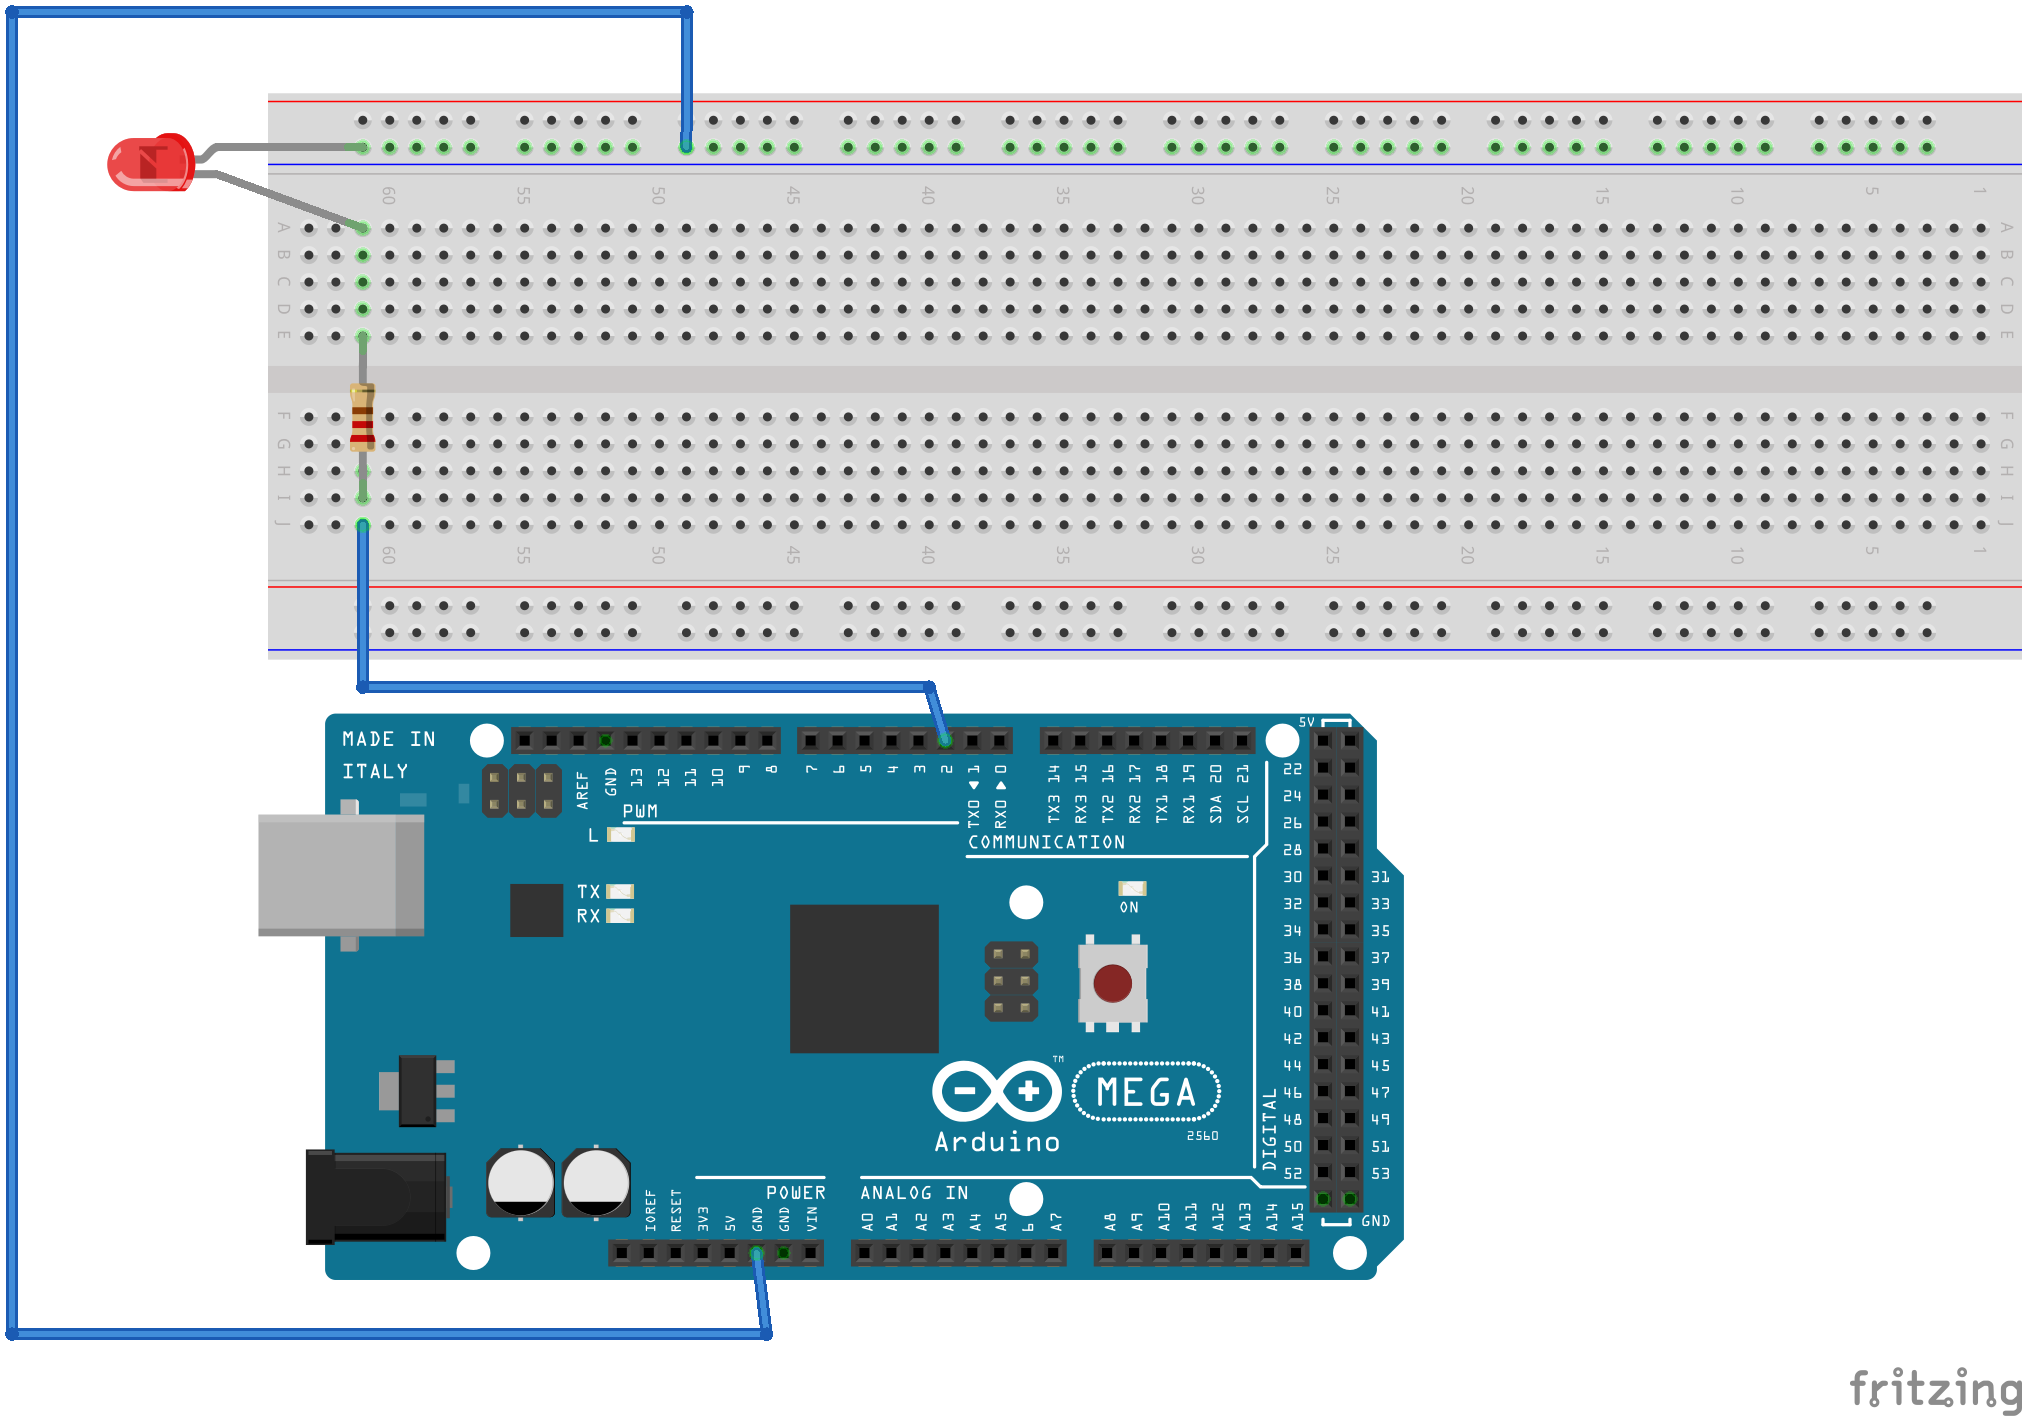
\includegraphics[width=12cm]{schematics/001-led}
  \caption{Пример подключения светодиода к Arduino Mega 2560 через макетную
    плату.}
  \label{fig:breadboard-led}
\end{figure}

\begin{itemize}
\item Черный провод подключен к Arduino и идёт на вывод ``GND'' (минус.)
\item Синий провод подключен к Arduino и идёт на вывод ``5V'' (плюс.)
\end{itemize}

\note{ Обратите внимание, что светодиоды (и некоторые другие элементы)
  подключаются к платформе Arduino через резистор --- как было сказано в разделе
  \ref{section:electronics-resistance}, резистор позволяет ограничивать ток в
  цепи, тем самым защищая электронные компоненты от преждевременного выхода из
  строя. }

В примере на рис. \ref{fig:breadboard-led} светодиод включится и будет постоянно
гореть, как только мы подадим питание на Arduino, так как плюсовой контакт
светодиода (анод) постоянно подаётся 5 Вольт.

%%%%%%%%%%%%%%%%%%%%%%%%%%%%%%%%%%%%%%%%%%%%%%%%%%%%%%%%%%%%%%%%%%%%%%%%%%%%%%%%
\section{Подключение Arduino к компьютеру}
Чтобы подключить Arduino к компьютеру вам потребуется сама платформа Ardu\-ino
(в нашем случае мы используем Arduino Mega 2560) и кабель стандарта USB-В.

Соедините Arduino с компьютером через USB-кабель. Вы увидите, как на плате
загорится светодиод ``ON''.

Теперь необходимо настроить Arduino IDE для работы с подключенной Ardu\-ino, для
этого нужно войти в панель ``Инструменты'' затем ``Плата'' -- в этом меню
необходимо выбрать вариант Arduino, с которой вы сейчас работаете, затем в
подменю ``Порт'' небходимо выбрать порт, к которому подключена Arduino.

\experiment{1}{Давайте попробуем переподключить плюсовой контакт светодиода на
  землю (\texttt{GND}.)  Светодиод должен погаснуть.  Почему?}

\experiment{1}{Теперь поменяем резистор в схеме на резистор с большим
  сопротивлением (например, 500 Ом.)  Как и почему изменилась яркость
  светодиода?}

\end{document}
